\section{Algoritmi di regressione lineari}

\subsection{Regressione semplice lineare}
Si chiama semplice perché prevede ingressi scalari (e non vettori di \emph{feature}). È lineare perché, dato un \emph{training set} di coppie $(x_i, y_i)$, cerca la miglior retta che ne approssima l'andamento.

La generica ipotesi ha espressione:
\begin{equation*}
 h(x) = \theta_0 + \theta_1 x
\end{equation*}
dove:
\begin{itemize}
  \item $\theta_0$ prende il nome di \emph{bias} e rappresenta l'intercetta con l'asse delle $y$;
  \item $\theta_1$ è il coefficiente angolare della retta desiderata.
\end{itemize}
Lo scopo della fase di \emph{training} è individuare i valori ottimi dei parametri $\theta_i$ (vedremo a breve cosa si intende per valori ottimi).

\subsection{Regressione multipla lineare}
È simile alla regressione semplice lineare, ma gli ingressi sono vettori di \emph{feature}.  Dunque non cerchiamo una retta, ma un iperpiano separatore, dalla generica espressione:
\begin{equation*}
  h(x) = \theta_0 + \sum_{i=1}^n \theta_i x_i.
\end{equation*}
Introducendo $x_0=1$ possiamo riscrivere la precedente come segue
\begin{equation*}
  h(x) = \sum_{i=0}^n \theta_i x_i = \theta^T \mathbf{x}
\end{equation*}
dove 
\begin{itemize}
  \item $\theta = {(\theta_0, \theta_1, \dots, \theta_n)}^T$ rappresenta il vettore dei parametri da apprendere durante la fase di addestramento;
  \item $n$ rappresenta la dimensione degli ingressi, cioè il numero di \emph{feature}. Notiamo che per $n$ ingressi occorre apprendere $n+1$ parametri $\theta_i$.
\end{itemize}

\subsubsection{Funzione costo}
Per individuare i valori ottimi dei $\theta_i$ costruiamo una funzione costo $J(\theta)$. Essa deve tener conto della differenza tra i valori di \emph{output} forniti dal \emph{training set} e gli stessi valori calcolati tramite l'ipotesi $h(x)$. Avrà quindi questa espressione:
\begin{equation}\label{eqJ_theta_semplice}
  J(\theta) = \frac{1}{2m} \sum_{i=1}^m (h_\theta(\mathbf{x^{(i)}})-y^{(i)})^2
\end{equation}
dove:
\begin{itemize}
  \item $m$ è il numero di istanze del \emph{training set};
  \item $\frac{1}{2m}$ è un fattore di normalizzazione, il coefficiente $2$ viene introdotto per semplificare le derivate parziali (vedi \autoref{sec:gradiente});
  \item $(h_\theta(\mathbf{x^{(i)}})-y^{(i)})$ è l'errore di predizione sul campione \emph{i-esimo}, calcolato come differenza tra l'\emph{output} stimato dal modello e quello letto dal \emph{training set}.
\end{itemize}
Elevando al quadrato e sommando ciascun errore si ottiene una funzione $J(\theta)$ quadratica  facilmente (e sicuramente) minimizzabile. Lo scopo della fase di apprendimento è quindi individuare per quali $\theta$ la funzione costo è minima:
\begin{equation*}
  \theta_{min} = \argmin_\theta( J(\theta)).
\end{equation*}

\subsection{Metodo delle equazioni normali}
Un primo approccio alla minimizzazione della funzione costo è quello analitico.
Definiamo innanzitutto una matrice $\mathbf{X}$ di dimensioni $m \times (n+1)$ in cui ciascuna riga rappresenta un ingresso nel \emph{training set}. Definiamo, inoltre, un vettore colonna $\mathbf{y}$ di $m$ elementi, ciascuno dei quali rappresenta l'uscita associata all'ingresso \emph{i-esimo} (nonché riga \emph{i-esima} di $\mathbf{X}$):

\begin{equation*}
\mathbf{X} = \begin{bmatrix}
 \mathbf{x^{(1)T}}\\
 \mathbf{x^{(2)T}}\\
 \vdots \\
  \mathbf{x^{(i)T}}\\
  \vdots \\
   \mathbf{x^{(m)T}}\\
\end{bmatrix} \qquad
\mathbf{y} = \begin{bmatrix}
 y^{(1)}\\
 y^{(2)}\\
 \vdots \\
 y^{(i)}\\
  \vdots \\
 y^{(m)}\\
\end{bmatrix}
\end{equation*}
La funzione costo può essere riscritta sotto forma di prodotto tra matrici:
\begin{equation*}
J(\theta) = \frac{1}{2} (\mathbf{X}\theta - \mathbf{y})^T (\mathbf{X}\theta - \mathbf{y}).
\end{equation*}
Cerchiamo il punto di minimo annullandone il gradiente:
\begin{equation*}
\nabla J(\theta) = \mathbf{X}^T\mathbf{X}\theta - \mathbf{X}^T \mathbf{y} = 0
\end{equation*}
da cui si ricava che
\begin{equation*}
\hat\theta = (\mathbf{X}^T\mathbf{X})^{-1} \mathbf{X}^T \mathbf{y}.
\end{equation*}
Questo metodo richiede il calcolo dell'inversa di $(\mathbf{X}^T\mathbf{X})$, di dimensioni $(n+1) \times (n+1)$. Quando il numero di \emph{feature} è piuttosto grande, questo calcolo diventa troppo costoso: tipicamente la complessità computazionale del calcolo dell'inversa è $\mathcal{O}(n^3)$ e questo può rendere il metodo delle equazioni normali anche più lento di metodi iterativi come la discesa a gradiente\footnote{\href{http://www.youtube.com/watch?v=B3vseKmgi8E}{{Coursera, Machine Learning (Andrew Ng), Lezione 4.6}}}. Per tale motivo, quando il numero di \emph{feature} è almeno nell'ordine di $10^5$, si preferiscono metodi numerici come quello della discesa del gradiente che analizzeremo in seguito. Il metodo delle equazioni normali, tuttavia, essendo analitico non richiede la determinazione empirica di alcun parametro (contrariamente a quanto accade con il \emph{learning rate} nella discesa a gradiente) e non è necessario effettuare alcun tipo di \emph{feature scaling} (di cui parleremo in \autoref{feature_scaling}).

In ultimo, consideriamo il caso in cui $\mathbf{X}^T\mathbf{X}$ non sia invertibile. Questo si verifica raramente, e se accade le cause più probabili sono due\footnote{\href{http://www.youtube.com/watch?v=0TMfGA3zQFQ}{Coursera, Machine Learning (Andrew Ng), Lezione 4.7}}:
\begin{itemize}
\item ci sono 2 o più \emph{feature} linearmente dipendenti, per cui è sufficiente eliminarle tutte tranne una;
\item il numero di esempi di addestramento è troppo basso rispetto al numero di \emph{feature}. Questo problema può essere risolto eliminando alcune \emph{feature} tramite tecniche di \emph{feature selection} oppure adottando tecniche di regolarizzazione.
\end{itemize}


\subsubsection{Dimostrazione}
Deriviamo ora le espressioni mostrate nel paragrafo precedente\footnote{Questa parte non è stata trattata a lezione, chi si fida dei risultati può saltarla senza problemi.}. Innanzitutto definiamo una funzione costo non normalizzata rispetto al numero di campioni, che useremo durante la dimostrazione\footnote{Minimizzare questa funzione costo o la sua variante normalizzata porta allo stesso risultato.}:
\begin{equation}\label{eq:J_sum}
J(\theta) = \frac{1}{2} \sum_{i=1}^m (h_\theta(\mathbf{x^{(i)}})-y^{(i)})^2.
\end{equation}
Si vede facilmente che la precedente è uguale a:
\begin{equation}\label{eq:J_matrix}
J(\theta) = \frac{1}{2} (\mathbf{X}\theta - \mathbf{y})^T (\mathbf{X}\theta - \mathbf{y}).
\end{equation}
Infatti è vero che:
\begin{equation*}
\mathbf{X}\theta - \mathbf{y} = \begin{bmatrix}
 1 & x_1^{(1)} & \dots & x_n^{(1)} \\
 1 & x_1^{(2)} & \dots & x_n^{(2)} \\
\vdots &\vdots &\ddots &\vdots  \\
1 & x_1^{(m)} & \dots & x_n^{(m)} \\
 \end{bmatrix}
 \begin{bmatrix}
 \theta_0 \\  \theta_1 \\ \vdots \\ \theta_n
 \end{bmatrix}
 -
  \begin{bmatrix}
 y^{(1)}\\  y^{(2)} \\ \vdots \\ y^{(m)}
 \end{bmatrix}
 =
 \begin{bmatrix}
 h_\theta(\mathbf{x^{(1)}}) - y^{(1)} \\
  h_\theta(\mathbf{x^{(2)}}) - y^{(2)} \\
  \vdots \\
   h_\theta(\mathbf{x^{(m)}}) - y^{(m)} \\
 \end{bmatrix}
\end{equation*}
E quindi:
\begin{dmath*}
(\mathbf{X}\theta - \mathbf{y})^T (\mathbf{X}\theta - \mathbf{y}) = \begin{bmatrix}
 (h_\theta(\mathbf{x^{(1)}}) - y^{(1)}) & 
  \dots &
  (h_\theta(\mathbf{x^{(m)}}) - y^{(m)}) \\
 \end{bmatrix}
 \begin{bmatrix}
 h_\theta(\mathbf{x^{(1)}}) - y^{(1)} \\
  \vdots \\
   h_\theta(\mathbf{x^{(m)}}) - y^{(m)} \\
 \end{bmatrix}
 = \sum_{i=1}^m (h_\theta(\mathbf{x^{(i)}})-y^{(i)})^2.
\end{dmath*}
Sostituendo la sommatoria in \autoref{eq:J_sum} con il prodotto tra matrici, si ottiene l'\autoref{eq:J_matrix}.
A noi interessa trovare il minimo della funzione costo, cioè il punto in cui si annulla il suo gradiente:
\begin{equation*}
\nabla J(\theta) = \begin{bmatrix}
\frac{ \partial J(\theta)}{\partial\theta_0} \\
\vdots \\
\frac{ \partial J(\theta)}{\partial\theta_k} \\
\vdots \\
\frac{ \partial J(\theta)}{\partial\theta_n} \\
 \end{bmatrix}=0
\end{equation*}
Similmente a quanto dimostreremo in seguito (\autoref{sec:gradiente}), si vede che la \emph{k-esima} derivata parziale del gradiente assume la seguente espressione:
\begin{dmath*}
\frac{ \partial J(\theta)}{\partial\theta_k}  = \sum_{i=1}^m (h_\theta(\mathbf{x^{(i)}})-y^{(i)})x_k^{(i)} = \begin{bmatrix}
 (h_\theta(\mathbf{x^{(1)}}) - y^{(1)}) &
  \dots &
  (h_\theta(\mathbf{x^{(m)}}) - y^{(m)}) \\
 \end{bmatrix}
 \begin{bmatrix}
 x^{(1)}_k \\
 \vdots \\
 x^{(m)}_k \\
 \end{bmatrix}
\end{dmath*}.
A questo punto riscriviamo per esteso l'espressione del gradiente\footnote{Ricordiamo che $x_0^{(i)}=1$ per $i=1,\dots,m$.}:
\begin{equation*}
\nabla J(\theta) = \begin{bmatrix}
\sum_{i=1}^m (h_\theta(\mathbf{x^{(i)}})-y^{(i)}) \\
\sum_{i=1}^m (h_\theta(\mathbf{x^{(i)}})-y^{(i)})x_1^{(i)} \\
\vdots \\
\sum_{i=1}^m (h_\theta(\mathbf{x^{(i)}})-y^{(i)})x_n^{(i)} \\
 \end{bmatrix}
\end{equation*}
Questa può essere riscritta come prodotto tra matrici:
\begin{dmath*}
\nabla J(\theta) = \begin{bmatrix}
1 & 1 & \dots  & 1 \\
 x_1^{(1)}  & x_1^{(2)} & \dots  & x_1^{(m)} \\

  \vdots & \vdots & \ddots & \vdots \\
   x_n^{(1)}  & x_n^{(2)} & \dots &  x_n^{(m)} \\
\end{bmatrix}
\begin{bmatrix}
 h_\theta(\mathbf{x^{(1)}}) - y^{(1)} \\
h_\theta(\mathbf{x^{(2)}}) - y^{(2)} \\
  \vdots \\
   h_\theta(\mathbf{x^{(m)}}) - y^{(m)} \\
\end{bmatrix}
= \mathbf{X}^T (\mathbf{X} \theta - \mathbf{y})
= \mathbf{X}^T \mathbf{X} \theta - \mathbf{X}^T  \mathbf{y}
\end{dmath*}
Adesso risolviamo l'equazione di annullamento del gradiente:
\begin{equation*}
\nabla J(\theta) = \mathbf{X}^T \mathbf{X} \theta - \mathbf{X}^T  \mathbf{y} = 0
\end{equation*}
dalla quale si ricava che
\begin{equation*}
\hat \theta = (\mathbf{X}^T\mathbf{X})^{-1} \mathbf{X}^T \mathbf{y}.
\end{equation*}

\subsection{Metodo della discesa del gradiente}\label{sec:gradiente}
Come già accennato, il metodo della discesa del gradiente consente di trovare il minimo di una funzione per via numerica. Noi lo applicheremo alla funzione costo.

Data una funzione, sono note alcune proprietà del suo gradiente:
\begin{enumerate}
  \item esso è un vettore che punta sempre nel verso in cui la pendenza della funzione aumenta;
  \item è esso stesso un indicatore della pendenza della curva.
\end{enumerate}
Dalle precedenti consegue che il gradiente è tanto più grande quanto maggiore è la pendenza della curva e punta nel verso in cui aumenta la pendenza.

\begin{esempio}
È facile riscontrare questo comportamento con un paraboloide:
\begin{equation*}
  y = f(x_1,x_2) = x_1^2 + x_2^2
\end{equation*}
Il gradiente è
\begin{equation*}
  \nabla(f(x_1,x_2))=(2x_1, 2x_2)
\end{equation*}
Calcolando il gradiente in un punto $P:(1,2)$ otteniamo
\begin{equation*}
  \nabla(f(1,2))=(2, 4)
\end{equation*}
il quale è un vettore parallelo  al piano su cui giace la curva di livello nel punto $P$, ha direzione perpendicolare alla tangente a tale curva in P e punta verso l'esterno del paraboloide, lì dove la pendenza aumenta.
\end{esempio}

Sfruttando queste conoscenze possiamo elaborare un metodo per aggiornare i coefficienti $\theta_i$ fino a raggiungere il minimo di $J(\theta)$. L'idea di base è quella di partire da $\theta_i$ casuali ed aggiornarli in maniera tale da spostarsi verso il minimo, cioè in verso opposto rispetto a quello del gradiente nel punto attuale (ricorda che ragioniamo su $J(\theta)$, quindi le $x^{(i)}$ sono solo coefficienti numerici, mentre le $\theta_i$ sono le variabili del problema). Per fare ciò si adotta la seguente regola di aggiornamento dei coefficienti:
\begin{equation*}
  \theta_k^{NEW} = \theta_k^{OLD} - \alpha \frac{ \partial J(\theta)}{ \partial \theta_k}
\end{equation*}

dove
\begin{itemize}
  \item $\theta_k^{NEW}$ rappresenta il nuovo valore del \emph{k-esimo} coefficiente, cioè quello che stiamo calcolando;
  \item $\theta_k^{OLD}$ è il valore dello stesso coefficiente all'iterazione precedente;
  \item $\alpha$ rappresenta un parametro detto \emph{learning rate}, il cui valore è positivo e tipicamente minore di $1$;
  \item $\frac{ \partial J(\theta)}{ \partial \theta_k}$ rappresenta la derivata parziale  della funzione costo rispetto al coefficiente \emph{k-esimo}.
\end{itemize}

Osserviamo il segno negativo prima della derivata parziale, poiché, come giustificato in precedenza, vogliamo spostarci nel verso opposto rispetto a quello del gradiente.
Notiamo, inoltre, che $\alpha$ è un fattore moltiplicativo il cui scopo è ``amplificare'' l'effetto del secondo addendo, esso influisce dunque sull'ampiezza degli incrementi/decrementi dovuti alla derivata parziale. Osserviamo però che:
\begin{itemize}
  \item un \emph{learning rate} troppo basso può rallentare l'agoritmo e portare a lunghi tempi di convergenza;
  \item un \emph{learning rate} troppo alto rischia di non farci trovare il minimo, poiché ``saltiamo'' da un lato all'altro della quadratica senza cadere nel centro.
\end{itemize}
In ultimo notiamo che il gradiente diminuisce man mano che ci avviciniamo al minimo, quindi all'inizio i decrementi subiti dai $\theta_i$ saranno più ampi, per poi diventare sempre più piccoli (ciò accadrebbe anche in assenza di $\alpha$).

Notiamo, in ultimo, che questo algoritmo funziona correttamente in assenza di minimi locali. Se questi ci fossero si potrebbe riavviare l'algoritmo più volte, partendo da diversi $\theta_i$ casuali, e vedere se il punto finale di convergenza rimane pressoché invariato o se l'algoritmo è incappato in minimi locali. Ovviamente nel caso della funzione costo definita in precedenza questo problema non si presenta.

In ultimo esplicitiamo le derivate parziali:
\begin{dmath*}
  \frac{\partial J(\theta)}{\partial \theta_k} 
  = \frac{\partial}{\partial \theta_k} \left( \frac{1}{2m} \sum_{i=1}^{m}(h_\theta(\mathbf{x^{(i)}})-y^{(i)})^2 \right)
  = \frac{1}{2m} \sum_{i=1}^{m}\frac{\partial }{\partial \theta_k}  \left ( h_\theta(\mathbf{x^{(i)}})-y^{(i)} \right)^2,
\end{dmath*}
ricordandoci che $ h(x)= \theta^T \mathbf{x}$
possiamo esaminare il singolo addendo della precedente sommatoria
\begin{dmath*}
  \frac{\partial}{\partial \theta_k}  \left(h_\theta(\mathbf{x^{(i)}})-y^{(i)}\right)^2 
  =  2\left(h_\theta(\mathbf{x^{(i)}})-y^{(i)}\right)\frac{\partial }{\partial \theta_k} h_\theta(\mathbf{x^{(i)}})
\end{dmath*}
dove 
\begin{dmath*}
  \frac{\partial}{\partial \theta_k} h_\theta(\mathbf{x^{(i)}}) 
  = \frac{\partial}{\partial \theta_k} \theta^T x^{(i)}
  =\frac{\partial}{\partial \theta_k} (\theta_0, \theta_1, \dots, \theta_k, \dots, \theta_n) (1, x^{(i)}_1,x^{(i)}_2, \dots, x^{(i)}_k, \dots, x^{(i)}_n)^T
  = (0, 0, \dots, 1, \dots, 0) (1, x^{(i)}_1,x^{(i)}_2, \dots, x^{(i)}_k, \dots, x^{(i)}_n)^T
  = x^{(i)}_k.
\end{dmath*}
Ricomponendo i passaggi otteniamo
\begin{dmath*}
  \frac{\partial}{\partial \theta_k}  \left(h_\theta(\mathbf{x^{(i)}})-y^{(i)}\right)^2 
  =  2\left(h_\theta(\mathbf{x^{(i)}})-y^{(i)}\right)x^{(i)}_k
\end{dmath*}
e tornando alla derivata parziale
\begin{dmath*}
  \frac{\partial J(\theta)}{\partial \theta_k} 
  = \frac{1}{2m} \sum_{i=1}^{m}\frac{\partial }{\partial \theta_k}  \left ( h_\theta(\mathbf{x^{(i)}})-y^{(i)} \right)^2
  = \frac{1}{m} \sum_{i=1}^m (h_\theta(\mathbf{x^{(i)}})-y^{(i)}) x^{(i)}_k.
\end{dmath*}
A questo punto possiamo esplicitare l'equazione di aggiornamento dei coefficienti:
\begin{equation*}
   \theta_k^{NEW} = \theta_k^{OLD} - \alpha \frac{1}{m} \sum_{i=1}^m (h_\theta(\mathbf{x^{(i)}})-y^{(i)}) x^{(i)}_k.\end{equation*}
   
\subsubsection{Batch gradient descent}
È un algoritmo che utilizza la regola di aggiornamento dei coefficienti precedentemente descritta e può essere sintetizzato così:
\begin{itemize}
  \item inizializza casualmente i $\theta_i$
  \item finché non raggiungi la condizione di convergenza aggiorna i coefficienti:
  \begin{equation*}
    \theta_k^{NEW} = \theta_k^{OLD} - \alpha \frac{1}{m} \sum_{i=1}^m (h(\mathbf{x^{(i)}})-y^{(i)}) x^{(i)}_k \qquad k = 0, 1, \dots, n
    \end{equation*}
  
\end{itemize}
La condizione di convergenza è tipicamente un valore massimo della funzione errore, al di sotto del quale ci accontentiamo del risultato ottenuto, o un numero massimo di iterazioni (oppure entrambe, in maniera tale che la seconda intervenga solo quando la prima non viene mai soddisfatta).

L'algoritmo si chiama \emph{batch} perché per aggiornare ciascun singolo $\theta_k$ usa tutte le istanze nel \emph{training set} (una sua variante, chiamata \emph{mini batch}, ne usa solo una porzione). I limiti di questo approccio emergono quando il \emph{training set} è molto grade e l'algoritmo tende ad essere lento (oltre a ciò, occorre caricare in memoria tutte le istanze per poter procedere nell'algoritmo, e ciò potrebbe essere impossibile su calcolatori modesti).

\subsubsection{Stochastic gradient descent}
A differenza dell'algoritmo \emph{batch}, la versione stocastica\footnote{\href{http://youtu.be/gdZxqnTKndE}{Coursera, Machine Learning (Andrew Ng), Lezione 17.2}} (anche detta ``incrementale'') aggiorna tutti i coefficienti dopo aver esaminato un singolo campione, solo in seguito passa al campione successivo. Di conseguenza occorre rivisitare leggermente la regola di aggiornamento dei pesi. 

L'algoritmo  può essere sintetizzato come segue:
\begin{itemize}
  \item inizializza casualmente i $\theta_i$
  \item ripeti fino a convergenza
  \begin{itemize}
    \item per i = 1, \dots, m
    \begin{itemize}
    \item per k=1, \dots, n
    \begin{equation*}
    \theta_k^{NEW} = \theta_k^{OLD} - \alpha (h(\mathbf{x^{(i)}})-y^{(i)}) x^{(i)}_k
    \end{equation*}
    \end{itemize}
  \end{itemize}
\end{itemize}

Notiamo che all'interno del ciclo \texttt{for} più interno ciascuna iterazione comporta l'aggiornamento di tutti i $\theta_i$ in base all'informazione proveniente da un singolo esempio. Questo implica che per ogni passo nel \texttt{for}, il punto attuale viene leggermente modificato tenendo conto di un solo esempio, quindi lo spostamento compiuto non va necessariamente nella direzione del minimo, ma cerca solo di fare un \emph{fitting} migliore verso l'istanza attualmente analizzata. A causa di ciò la ``traiettoria'' con cui l'algoritmo si sposta verso il minimo non è diretta come per la versione \emph{batch}, ma sembra più casuale. Per lo stesso motivo l'algoritmo potrebbe ritrovarsi a girare attorno al minimo senza raggiungerlo, pur restando in un intorno ragionevole. Tuttavia, poiché ciascun aggiornamento dei $\theta_i$ non implica la scansione di tutto il \emph{training set}, l'algoritmo converge più velocemente (quando il \emph{set} è grande).

La differenza sostanziale è questa: mentre nella versione \emph{batch} occorre analizzare tutto il \emph{training set} per compiere un piccolo passo, con quella \emph{stochastic} si aggiorna leggermente il punto per ogni singola istanza che si analizza ed al termine dell'intero ciclo \texttt{for} lo spostamento verso il minimo potrebbe essere più significativo di quanto accadrebbe con una singola iterazione di algoritmo \emph{batch}. Inoltre, nella variante stocastica la condizione di convergenza può essere verificata dopo ogni piccolo aggiornamento e non necessariamente dopo un intero ciclo.

\subsubsection{Nota sull'aggiornamento dei coefficienti}
Riprendiamo la formula di aggiornamento dei coefficienti:

\begin{equation*}
  \theta_k^{NEW} = \theta_k^{OLD} - \alpha \frac{ \partial J(\theta)}{ \partial \theta_k}
\end{equation*}

È importante notare che la derivata parziale dipende, ovviamente, da $h_\theta(x)$, la quale cambia al variare dei $\theta_i$. Quando implementiamo concretamente questa regola, occorre calcolare prima tutte le derivate parziali, mantenendo invariati i coefficienti $\theta_i$, memorizzare i nuovi coefficienti in variabili temporanee e poi aggiornare contemporaneamente tutti i coefficienti\footnote{\href{http://www.youtube.com/watch?v=eikJboPQDT0}{Coursera, Machine Learning (Andrew Ng), Lezione 2.5}}, ovvero:

\begin{gather*}
temp1 := \theta_1 - \alpha \frac{ \partial J(\theta)}{ \partial \theta_1}; \\
temp2 := \theta_2 - \alpha \frac{ \partial J(\theta)}{ \partial \theta_2}; \\
\dots \\
\theta_1 := temp1; \\
\theta_2 := temp2;\\
\end{gather*}
La maniera \emph{sbagliata} di fare ciò è la seguente:
\begin{gather*}
\theta_1 := \theta_1 -\alpha \frac{ \partial J(\theta)}{ \partial \theta_1}; \\
\theta_2 := \theta_2 - \alpha \frac{ \partial J(\theta)}{ \partial \theta_2}; \\
\dots
\end{gather*}
Così facendo, infatti, abbiamo aggiornato $\theta_1$ e per aggiornare $\theta_2$ calcoliamo la derivata di $J(\theta)$ con \emph{il nuovo valore di $\theta_1$}, che è diverso da ciò che dovremmo fare. Questa variante, che abbiamo etichettato come errata, potrebbe funzionare, ma non è il \emph{gradient descent} e potrebbe comportarsi diversamente da come ci aspettiamo.

\subsection{Interpretazione probabilistica della regressione lineare}

Siano $(\mathbf{x^{(i)}},y^{(i)})$ le $m$ istanze di un \emph{training set}. Quando applichiamo la regressione lineare cerchiamo un'ipotesi $ h(\mathbf{x}) = \theta^T \mathbf{x}$ che approssimi la relazione tra vettori di \emph{feature} ed \emph{output}. Nel fare ciò, ciascun valore di \emph{output} del \emph{training set} potrà essere espresso come somma di un valore calcolato tramite l'ipotesi ed un errore: \begin{equation}\label{eq:e}
   y^{(i)}=\theta^T \mathbf{x^{(i)}}+e^{(i)}.
 \end{equation}
 Assumiamo che i campioni siano indipendenti, e dunque lo saranno anche gli errori $e^{(i)}$ che assumiamo essere anche identicamente distribuiti con distribuzione normale, a valor medio nullo e varianza $\sigma^2$: 
 \begin{equation}\label{eqp(e)}
  p(e^{(i)}) = \mathcal{N}(0, \sigma^2) = \frac{1}{\sqrt{2 \pi} \sigma } e ^{-\frac{(e^{(i)})^2}{2 \sigma^2}} \qquad i=1 \dots m.\end{equation}   
Fissato un modello, e dunque i parametri $\theta$, la probabilità che l'ingresso $\mathbf{x^{(i)}}$ generi l'uscita $y^{(i)}$ avrà la stessa distribuzione dell'errore $e^{(i)}$. Sostituendo $e^{(i)}=y^{(i)}- \theta^T \mathbf{x^{(i)}}$ (dall'\autoref{eq:e}) nell'\autoref{eqp(e)} otteniamo:

 \begin{equation*}
   p(y^{(i)}|\mathbf{x^{(i)}}; \theta) = \frac{1}{\sqrt{2 \pi} \sigma } e ^{-\frac{(y^{(i)}-\theta^T \mathbf{x^{(i)}})^2}{2 \sigma^2}} \qquad i=1 \dots m.\end{equation*}

A questo punto vogliamo trovare un'espressione della probabilità che, fissati i parametri $\theta$, al \emph{set} di ingressi $\mathbf{x^{(i)}}$ corrispondano le uscite $y^{(i)}$ per ogni $i=1,\dots,m$. Questa probabilità viene chiamata ``verosimiglianza'' (\emph{likelihood}) ed è così espressa:
\begin{equation*}
  L(\theta) = L(\theta;\mathbf{X};\mathbf{y})=p(\mathbf{y}|\mathbf{X};\theta) 
\end{equation*}
dove
\begin{itemize}
  \item $\mathbf{X}$ rappresenta l'insieme degli \emph{input} (possiamo vederlo come una matrice $m \times (n+1)$),
  \item $\mathbf{y}$ rappresenta il vettore delle uscite (di dimensioni $m \times 1$).
\end{itemize}
 Avendo ipotizzato che tutti i campioni siano indipendenti, la probabilità dell'evento congiunto è la seguente:
 \begin{equation*}
   L(\theta) =
    p(\mathbf{y}|X;\theta) 
    = \prod_{i=1}^m p(y^{(i)}|\mathbf{x^{(i)}};\theta)
    = \prod_{i=1}^m \frac{1}{\sqrt{2 \pi} \sigma } e ^{-\frac{(y^{(i)}-\theta^T \mathbf{x^{(i)}})^2}{2 \sigma^2}}
 \end{equation*}
Adottando il criterio di ``massima verosimiglianza'' siamo interessati al vettore $\theta$ che massimizza la funzione $L(\theta)$. Così facendo stiamo cercando i $\theta_i$ che danno vita all'ipotesi che ha maggior probabilità di restituire le uscite note quando si inseriscono i corrispondenti dati in \emph{input}.
Cerchiamo quindi
\begin{equation*}
  \hat\theta = \argmax_\theta L(\theta),
\end{equation*}
e poiché la funzione logaritmo è monotona crescente e non altera il punto di massimo, possiamo riformulare  il problema come segue:
\begin{equation*}
  \hat\theta = \argmax_\theta L(\theta) = \argmax_\theta \log  L(\theta) = \argmax_\theta l(\theta)
\end{equation*}
dove $\log L(\theta)=l(\theta)$.
Questa formulazione consente di ``trasformare'' la produttoria in una sommatoria, più facile da gestire da un punto di vista computazionale:
\begin{dmath*}
  l(\theta) = \log \prod_{i=1}^m p(y^{(i)}|\mathbf{x^{(i)}};\theta)
  = \sum_{i=1}^m \log\frac{1}{\sqrt{2\pi}\sigma}e^{-\frac{(y^{(i)}-\theta^T \mathbf{x^{(i)}})^2}{2\sigma^2}}
  = \sum_{i=1}^m \left( \log\frac{1}{\sqrt{2\pi}\sigma} + \log e ^{-\frac{(y^{(i)}-\theta^T \mathbf{x^{(i)}})^2}{2\sigma^2}} \right)
  = m \log\frac{1}{\sqrt{2\pi}\sigma} - \sum_{i=1}^m \frac{(y^{(i)}-\theta^T \mathbf{x^{(i)}})^2}{2\sigma^2}
  = m \log\frac{1}{\sqrt{2\pi}\sigma} - \frac{1}{2\sigma^2} \sum_{i=1}^m (y^{(i)}-\theta^T \mathbf{x^{(i)}})^2
\end{dmath*}
Ritorniamo al problema di massimizzazione:
\begin{dmath*}
  \max_\theta l(\theta)= \max_\theta \left( m \log\frac{1}{\sqrt{2\pi}\sigma} - \frac{1}{2\sigma^2} \sum_{i=1}^m (y^{(i)}-\theta^T \mathbf{x^{(i)}})^2\right)
  = \max_\theta \left(- \frac{1}{2\sigma^2} \sum_{i=1}^m (y^{(i)}-\theta^T \mathbf{x^{(i)}})^2\right)=
   \max_\theta \left( -\frac{1}{2} \sum_{i=1}^m (y^{(i)}-\theta^T \mathbf{x^{(i)}})^2\right)
  = \min_\theta  \left( \frac{1}{2} \sum_{i=1}^m (y^{(i)}-\theta^T \mathbf{x^{(i)}})^2\right).
\end{dmath*}
Confrontando l'ultima espressione con l'errore $J(\theta)$ (\autoref{eqJ_theta_semplice}) e notiamo che il problema è identico, dato che l'unica differenza tra le due minimizzazioni è una costante di normalizzazione non influente ai fini del risultato.

\begin{dmath}\label{eqJ_theta}
 \min_\theta \left(\frac{1}{2m} \sum_{i=1}^m (h(\mathbf{x^{(i)}})-y^{(i)})^2\right) =
 \min_\theta  \left( \frac{1}{2} \sum_{i=1}^m (y^{(i)}-\theta^T \mathbf{x^{(i)}})^2\right)
\end{dmath}

\subsection{Modelli lineari generalizzati (GLM)}
A volte la linearità dei modelli esaminati può essere limitante. Ad esempio, quando i dati del \emph{training set} non sono linearmente separabili, un modello lineare è del tutto inefficace. In tal caso, prima di passare a modelli non lineari, potrebbe essere interessante utilizzare delle \emph{funzioni base}.

\subsubsection{Funzioni base}
Le funzioni base rappresentano trasformazioni non lineari che applichiamo a ciascun vettore di ingresso. Esse, tipicamente, aumentano il numero di \emph{feature} e, tramite l'introduzione di non-linearità nei dati stessi, consentono di usare semplici modelli lineari per la classificazione.

Con riferimento alla regressione lineare, in condizioni normali l'ipotesi applicata ad un singolo ingresso è:
\begin{equation*}
h(\mathbf{x^{(i)}})= \sum_{j=1}^m \theta_j x_j^{(i)}=\theta^T \mathbf{x^{(i)}}.
\end{equation*}
Per introdurre una non-linearità possiamo avvalerci di una funzione base $\phi(x)$ che applichiamo all'ingresso $x^{(i)}$. Il risultato ($\phi(x^{(i)})$) sarà un vettore con più di $n$ componenti, ottenute tramite combinazione non lineare delle $n$ di partenza. Applichiamo quindi l'ipotesi (lineare) a tali vettori:
\begin{equation*}
h(\mathbf{x^{(i)}})= \sum_{j=1}^m \theta_j \phi(\mathbf{x^{(i)}})_j=\theta^T \boldsymbol{\phi}(\mathbf{x^{(i)}}).
\end{equation*}

\begin{esempio}
Una possibile funzione di base potrebbe associare ad un ingresso a 3 dimensioni $<x_1, x_2, x_3>$ un vettore a 9 dimensioni, così formato:
\begin{equation*}
<x_1, x_2, x_3, x_1 x_2, x_2 x_3, x_1 x_3, x_1^2, x_2^2, x_3^2>.
\end{equation*}
\end{esempio}

\section{Algoritmi di classificazione lineari}

\subsection{Regressione logistica}
Il modello è nella forma:
\begin{equation*}
h_\theta(\mathbf{x}) = \frac{1}{1+e^{-\theta^T \mathbf{x}}}
\end{equation*}
Poiché la funzione logistica varia tra 0 ed 1, possiamo dare un'interpretazione probabilistica alla sua uscita. Fissata una soglia (\emph{threshold}) fissiamo la classe di appartenenza a seconda che $h_\theta(x)$ sia maggiore o uguale alla soglia (classe 1) o minore (classe 0).

\begin{equation*}
y=\begin{cases} 1  \qquad \mbox{se }  h_\theta(\mathbf{x})\geq threshold \\
0 \qquad \mbox{se } h_\theta(\mathbf{x})< threshold 
\end{cases}
\end{equation*}

\subsubsection{Funzione costo}
Similmente a quanto fatto per la regressione lineare, individuiamo un'espressione della funzione costo che tenga conto della differenza tra le uscite reali e quelle predette tramite il modello. 
Per trovare tale espressione calcoliamo direttamente la funzione \emph{likelihood} ed applichiamo l'ipotesi di massima verosimiglianza (cioè massimiziamo la funzione di verosimiglianza).

Ricordiamo che $L(\theta)$ rappresenta la probabilità che, fissati i parametri $\theta$, agli ingressi $x^{(i)}$ corrispondano le uscite $y^{(i)}$ note, ed assumiamo che i campioni di addestramento siano indipendenti ed identicamente distribuiti:


\begin{equation}\label{eql_logistica}
   L(\theta) = L(\theta;X;\mathbf{y})=
    p(\mathbf{y}|X;\theta) 
    = \prod_{i=1}^m p(y^{(i)}|\mathbf{x^{(i)}};\theta).
 \end{equation}

Resta da capire quale sia la distribuzione di ciascun campione. Notiamo che l'uscita $y^{(i)}$ è binaria, quindi abbiamo due soli possibili eventi ($y^{(i)}=1$ e $y^{(i)}=0$), siamo quindi di fronte ad una distribuzione di Bernoulli $\mathcal{B}(p)$, dove $p$ rappresenta la probabilità dell'evento $y^{(i)}=1$ che ci apprestiamo a determinare. Abbiamo già detto che l'uscita della funzione logistica è compresa tra 0 ed 1, possiamo quindi interpretarla come la probabilità che all'ingresso $x^{(i)}$ corrisponda $y^{(i)}=1$. Ad esempio, data una $x$ in ingresso ad un modello ``perfetto'' la sua uscita dovrebbe essere $0$ o $1$, ma il nostro modello ci restituisce $h_\theta(x)=0.7$; dovendo decidere se $y$ sia $0$ o $1$, concludiamo che c'è il 70\% di probabilità che sia $1$. 
Riepiloghiamo dicendo che:
\begin{equation*}
\begin{cases}
p(y^{(i)}=1|\mathbf{x^{(i)}};\theta) = h_\theta(\mathbf{x^{(i)}})  \\
p(y^{(i)}=0|\mathbf{x^{(i)}};\theta) = 1 - h_\theta(\mathbf{x^{(i)}})
\end{cases}
\end{equation*}
che può essere scritto in maniera compatta come segue:
\begin{equation*}
p(y^{(i)}|\mathbf{x^{(i)}};\theta) = h_\theta(\mathbf{x^{(i)}})^{y^{(i)}} \cdot (1 - h_\theta(\mathbf{x^{(i)}}))^{1-y^{(i)}}.
\end{equation*}
Sostituiamo quest'ultima nell'\autoref{eql_logistica}:
\begin{equation*}
 L(\theta) = \prod_{i=1}^m h_\theta(\mathbf{x^{(i)}})^{y^{(i)}} \cdot (1 - h_\theta(\mathbf{x^{(i)}}))^{1-y^{(i)}}
\end{equation*}
e, come già fatto nella regressione lineare, passiamo al logaritmo:
\begin{dmath*}
 l(\theta) = \log\prod_{i=1}^m h_\theta(\mathbf{x^{(i)}})^{y^{(i)}} \cdot (1 - h_\theta(\mathbf{x^{(i)}}))^{1-y^{(i)}}
 = \sum_{i=1}^m \left( {y^{(i)}}\log{h_\theta(\mathbf{x^{(i)}})} + (1-y^{(i)})
 \log{(1 - h_\theta(\mathbf{x^{(i)}}))} \right)
\end{dmath*}.
Questa è la funzione che ci interessa massimizzare, nel dettaglio, però, minimizziamo il suo opposto  normalizzato rispetto al numero di campioni di addestramento (che prende il nome di \emph{cross entropy error function}):

 \begin{equation*}
 J(\theta) = -\frac{1}{m}\sum_{i=1}^m \left( {y^{(i)}}\log{h_\theta(\mathbf{x^{(i)}})} + (1-y^{(i)})
 \log{(1 - h_\theta(\mathbf{x^{(i)}}))} \right).
\end{equation*}
In conclusione, quindi, ci interessa il $\theta$ ottimo che minimizzi la precedente:
\begin{equation*}
  \hat\theta = \argmin_\theta J(\theta).
\end{equation*}

La funzione costo appena definita non può essere studiata da un punto di vista analitico, ma possiamo vedere quale contributo fornisce all'errore ciascun addendo:
 \begin{equation*}
  e^{(i)} = {y^{(i)}}\log{h_\theta(\mathbf{x^{(i)}})} + (1-y^{(i)})
 \log{(1 - h_\theta(\mathbf{x^{(i)}}))}
\end{equation*}
dove $e^{(i)}$ rappresenta il contributo all'errore apportato da un \emph{i-esimo} campione di addestramento.
 Distinguamo due casi:
\begin{itemize}
\item campione classificato come classe 1  ($y^{(i)}=1$);
\item campione classificato come classe 0 ($y^{(i)}=0$).
\end{itemize}
Nel primo caso, il singolo addendo assume l'espressione:

 \begin{equation*}
 e^{(i)}=-\log{h_\theta(\mathbf{x^{(i)}})} 
 \end{equation*}
 In \autoref{fig:errori_logistica} (linea rossa) è mostrato il suo andamento, concludiamo che:
\begin{itemize}
\item se il classificatore restituisce un valore basso, l'errore commesso classificandolo come 1 ($y^{(i)}=1$) sarà alto. Al limite accade che:
\begin{equation*}
h_\theta(\mathbf{x^{(i)}}) = 0 \Rightarrow e^{(i)} \rightarrow \infty
\end{equation*}
\item se il classificatore restituisce un valore alto, l'errore commesso classificandolo come 1 ($y^{(i)}=1$) sarà basso:
\begin{equation*}
h_\theta(\mathbf{x^{(i)}}) = 1 \Rightarrow e^{(i)} \rightarrow 0
\end{equation*}
\end{itemize}
Nel secondo caso ($y^{(i)}=0$), il contributo del singolo campione sarà:
\begin{equation*}
 e^{(i)}=-\log{(1-h_\theta(\mathbf{x^{(i)}}))} 
 \end{equation*}
In \autoref{fig:errori_logistica} (linea blu) è mostrato il suo andamento, concludiamo che:
\begin{itemize}
\item se il classificatore restituisce un valore basso, l'errore commesso classificandolo come 0 ($y^{(i)}=0$) sarà basso. Al limite accade che:
\begin{equation*}
h_\theta(\mathbf{x^{(i)}}) = 0 \Rightarrow e^{(i)} \rightarrow 0
\end{equation*}
\item se il classificatore restituisce un valore alto, l'errore commesso classificandolo come 0 ($y^{(i)}=0$) sarà alto:
\begin{equation*}
h_\theta(\mathbf{x^{(i)}}) = 1 \Rightarrow e^{(i)} \rightarrow \infty
\end{equation*}
\end{itemize}

\begin{figure}[]
\centering
  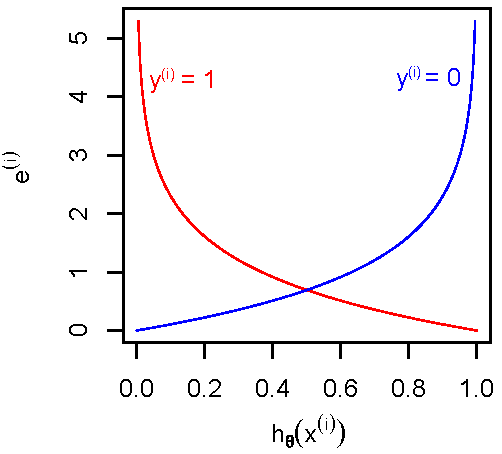
\includegraphics[width=0.5\columnwidth]{images/errori_logistica}
  \caption{Contributi all'errore nella regressione logistica}
  \label{fig:errori_logistica}
\end{figure}

\subsection{Metodo della discesa del gradiente}
Poiché non esiste un metodo analitico per minimizzare la funzione costo, l'unica l'alternativa è un metodo numerico, come quello basato sulla discesa del gradiente. Come già visto, questo metodo si basa sulla seguente regola di aggiornamento dei pesi:
\begin{equation*}
  \theta_k^{NEW} = \theta_k^{OLD} - \alpha \frac{ \partial J(\theta)}{ \partial \theta_k}.
\end{equation*}
Si vede facilmente che per la derivata della funzione logistica vale la seguente proprietà:
\begin{equation*}
g'(z) = \frac{\partial}{\partial z}\left( \frac{1}{1+e^{-z}}\right)=g(z)(1-g(z)).
\end{equation*}
Sfruttando la precedente nel calcolo delle derivate di $J(\theta)$ si vede che la regola di aggiornamento dei pesi è identica a quella della regressione lineare, cioè:
\begin{equation*}
   \theta_k^{NEW} = \theta_k^{OLD} - \alpha \frac{1}{m} \sum_{i=1}^m (h(x^{(i)})-y^{(i)}) x^{(i)}_k.\end{equation*}
Essa può essere applicata sia per il \emph{batch gradient descent} che per le sue varianti stocastiche.

\subsubsection{Derivazione della regola di aggiornamento dei pesi}\label{sec:dim_log_regr}
Vediamo ora quali sono i passaggi che portano all'espressione della regola di aggiornamento dei pesi\footnote{Approfondimento non trattato a lezione}. Come già detto, la derivata della funzione logistica gode della seguente proprietà:
\begin{equation*}
g'(z) =g(z)(1-g(z)).
\end{equation*}
Partendo da essa, calcoliamo la derivata parziale di $h_\theta(x)$, che tornerà utile in seguito:
\begin{equation*}
\frac{\partial h_\theta(x)}{\partial \theta_k} = h_\theta(x) (1-h_\theta(x)) \frac{\partial (\theta^T x)}{\partial \theta_k}
\end{equation*}
dove, come già visto in \autoref{sec:gradiente}, risulta che:
\begin{equation*}
\frac{\partial (\theta^T x)}{\partial \theta_k} = x_k
\end{equation*}
e quindi
\begin{equation*}
\frac{\partial h_\theta(x)}{\partial \theta_k} = h_\theta(x) (1-h_\theta(x)) x_k.
\end{equation*}
Passiamo ora al calcolo della derivata parziale di $J(\theta)$:

 \begin{equation}\label{eq:delta_j}
 \frac{\partial J(\theta)}{\partial \theta_k} = -\frac{1}{m}\sum_{i=1}^m \left( {y^{(i)}} \frac{\partial}{\partial \theta_k}(\log{h_\theta(x^{(i)})}) + (1-y^{(i)})
 \frac{\partial}{\partial \theta_k}(\log{(1 - h_\theta(x^{(i)}))}) \right).
\end{equation}
Esaminiamo separatamente le due derivate:
\begin{equation*}
\frac{\partial}{\partial \theta_k}\log{h_\theta(x^{(i)})} = \frac{1}{h_\theta(x^{(i)})} h_\theta(x^{(i)}) (1-h_\theta(x^{(i)})) x_k^{(i)} =  (1-h_\theta(x^{(i)})) x_k^{(i)}
\end{equation*}

\begin{equation*}
\frac{\partial}{\partial \theta_k}\log{(1 - h_\theta(x^{(i)}))} = \frac{1}{1- h_\theta(x^{(i)})} (-h_\theta(x^{(i)})) (1-h_\theta(x^{(i)})) x_k^{(i)} =  -h_\theta(x^{(i)}) x_k^{(i)}
\end{equation*}
Sostituiamo le precedenti nell'\autoref{eq:delta_j}, raccogliamo $x_k$ e sviluppiamo il prodotto per ottenere la derivata finale:

 \begin{dmath*}
 \frac{\partial J(\theta)}{\partial \theta_k} = -\frac{1}{m}\sum_{i=1}^m \left( {y^{(i)}} (1-h_\theta(x^{(i)})) x_k^{(i)} + (1-y^{(i)})
 (-h_\theta(x^{(i)})) x_k^{(i)} \right) 
 =-\frac{1}{m}\sum_{i=1}^m \left( {y^{(i)}} (1-h_\theta(x^{(i)})) + (1-y^{(i)})
 (-h_\theta(x^{(i)})) \right) x_k^{(i)}  
 = \frac{1}{m}\sum_{i=1}^m \left( h_\theta(x^{(i)}) - y^{(i)} \right) x_k^{(i)}  
\end{dmath*}

\subsection{Regressione logistica: caso multiclasse}
Con la regressione logistica siamo in grado di realizzare un classificatore binario. Se le classi sono più di due, si possono adottare due approcci:
\begin{enumerate}
\item usare una funzione logistica a più livelli (che non approfondiremo);
\item usare più funzioni logistiche in un approccio \emph{one-vs-all}, che ci apprestiamo ad approfondire.
\end{enumerate}
Supponiamo di dover distinguere $n$ classi, per farlo addestreremo $n$ classificatori (quindi avremo $n$ funzioni logistiche) ciascuno dei quali sarà in grado di identificare come classe 1 una classe desiderata, e tutte le altre $n-1$ saranno riconosciute come classe 0. Una volta addestrati gli $n$ classificatori, per classificare un nuovo ingresso lo diamo in \emph{input} a tutte le funzioni logistiche, ciascuna restituirà un valore tra 0 ed 1, quello più alto determinerà la classe di appartenenza dell'ingresso (cioè ci dirà quale classificatore ha dato la risposta più alta, presumibilmente quello specializzato sulla reale classe di appartenenza dell'ingresso). Di fatto in questo approccio interpretiamo l'uscita dell'\emph{i-esimo} classificatore come la probabilità che l'ingresso appartenga alla classe \emph{i-esima}.

\subsection{Regolarizzazione}
Uno dei problemi in cui è possibile incorrere è l'\emph{overfitting} e tramite la ``regolarizzazione'' possiamo evitarlo. 

L'idea di base è che, fissato il grado di un modello, il suo andamento sarà tanto più oscillatorio quanto più grandi saranno i $\theta_i$. La regolarizzazione, quindi, si propone di prevenire l'\emph{overfitting} penalizzando i $\theta_i$ grandi, senza agire direttamente sul grado del modello.

\subsubsection{Regolarizzazione con norma $\ell^2$}\label{sec:regolarizzazione_l2}

Il concetto di base è molto semplice: sommiamo alla funzione costo un qualcosa che penalizzi i $\theta_i$ grandi, nella fattispecie il nostro ``qualcosa'' è il quadrato della norma in modulo 2 del vettore 
 $\theta$ (escluso $\theta_0$ poiché è l'intercetta e non contribuisce all'andamento della funzione).

Nel caso della regressione lineare, la funzione costo regolarizzata prende il nome di \emph{Ridge Regression} ed è la seguente:
\begin{equation}\label{eqJ_theta}
  J(\theta) = \frac{1}{2m} \left(\sum_{i=1}^m (h(x^{(i)})-y^{(i)})^2 + \lambda \sum_{j=1}^n\theta_j^2\right)
\end{equation}
dove:
\begin{itemize}
\item $\sum_{j=1}^n\theta_j^2 = ||\theta||_2^2$; sommare questo contributo è equivalente a minimizzare $J(\theta)$ originale ponendo un vincolo sul valore massimo della norma;
\item $\lambda$ è detto parametro di regolarizzazione e determina l'influenza del fattore di regolarizzazione: più è grande, più piccoli saranno i $\theta$ e più smussata sarà l'ipotesi.
\end{itemize}
Nel caso della regressione logistica, questo approccio porta a riformulare la funzione costo come segue:
 \begin{equation*}
 J(\theta) = -\frac{1}{m}\sum_{i=1}^m \left( {y^{(i)}}\log{h_\theta(x^{(i)})} + (1-y^{(i)})
 \log{(1 - h_\theta(x^{(i)}))} \right) + \frac{\lambda}{2m}\sum_{j=1}^n\theta_j^2.
\end{equation*}
In maniera simile a quanto già fatto, possiamo calcolare le derivate delle funzioni costo regolarizzate e dedurre la regola di aggiornamento dei pesi. Si vede facilmente che, sia nel caso di regressione lineare che logistica, essa diventa:
\begin{gather*}\begin{cases}
\displaystyle\theta^{NEW}_0 = \theta^{OLD}_0 - \alpha \frac{1}{m} \sum_{i=1}^m \left(h_\theta(x^{(i)}) - y^{(i)}\right)x_0^{(i)} \\
\displaystyle\theta^{NEW}_k = \theta^{OLD}_k - \alpha \left[ \frac{1}{m} \sum_{i=1}^m \left(h_\theta(x^{(i)}) - y^{(i)}\right)x_k^{(i)}+\frac{\lambda}{m}\theta_k\right] \quad k=1,2,\dots,n
\end{cases}
\end{gather*}
La regola di aggiornamento di $\theta_0$ rimane invariata, come ci aspetteremmo sapendo che esso non è coinvolto nella regolarizzazione. Per tutti gli altri coefficienti possiamo riscrivere la regola come segue:
\begin{equation*}
\displaystyle\theta^{NEW}_k = \theta^{OLD}_k \left(1- \alpha\frac{\lambda}{m}\right) - \alpha \frac{1}{m} \sum_{i=1}^m \left(h_\theta(x^{(i)}) - y^{(i)}\right)x_k^{(i)} \quad k=1,2,\dots,n
\end{equation*}
Notiamo che la seconda parte della regola è identica alla versione senza regolarizzazione. In condizioni ``tipiche'' accade che $\alpha<1$, $\lambda > 0$ ed $m$ è piuttosto grande. Questo fa sì che il termine $\left(1- \alpha\frac{\lambda}{m}\right)$ sia minore di $1$. Ciò ci fornisce un'interessante interpretazione della nuova regola di aggiornamento. Infatti è come se l'algoritmo aggiornasse $\theta_k$ applicando la classica regola (senza regolarizzazione) a partire da una versione scalata del precedente valore di $\theta_k$ (poiché viene moltiplicato per una quantità minore di $1$).

\subsubsection{Regolarizzazione con norma $\ell^1$}
Un'ulteriore tecnica di regolarizzazione (detta \emph{lasso}) prevede di usare la norma $\ell^1$ piuttosto che il quadrato della norma $\ell^2$. 
Le espressioni precedenti rimangono invariate, ad eccezione dell'ultima sommatoria che viene sostituita da:
\begin{equation*}
\ell^1 = \sum_{j=1}^n|\theta_j|.
\end{equation*}
Questo tipo di sostituzione, però, implica che la nuova funzione costo $J(\theta)$ non sia più derivabile con continuità (a causa di $\ell^1$). 

Ma allora perché preferire $\ell^1$ ad $\ell^2$?

\subsubsection{$\ell^2$ vs $\ell^1$}
Le persone serie (non noi) hanno dimostrato le seguenti conclusioni.

\begin{figure}[]
\centering
  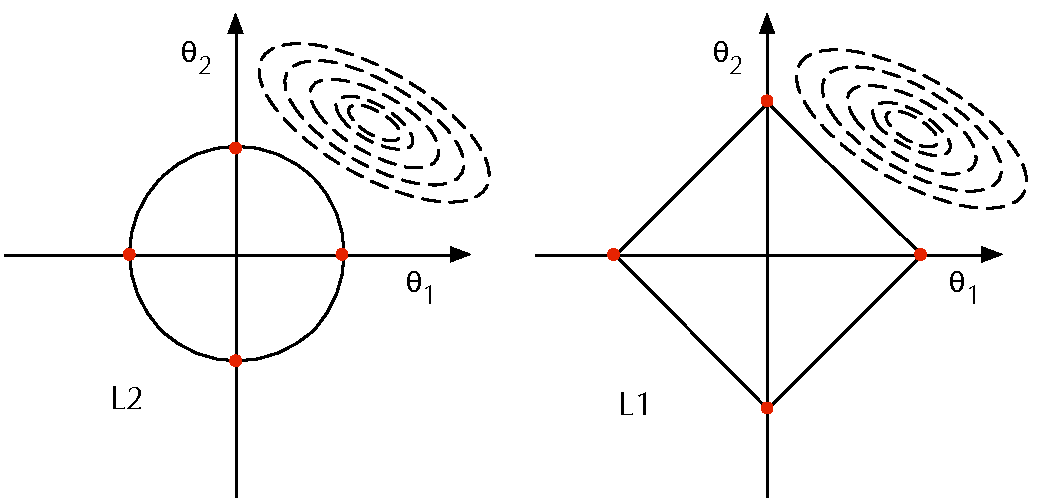
\includegraphics[width=\columnwidth]{images/norme}
  \caption{Regolarizzazione con norma $\ell^1$ ed $\ell^2$}
  \label{fig:norme}
\end{figure}

Come già detto, l'introduzione della norma nella funzione costo equivale ad imporre un limite al suo valor massimo. Possiamo quindi riscrivere i due problemi come segue (ignoriamo i fattori di normalizzazione $m$ al denominatore, senza che ciò cambi i risultati):

\begin{gather}
\text{Norma }\ell^2:
\quad \min\sum_{i=1}^m(\dots)^2 \\
\qquad \text{s.t.} \qquad ||\theta||_2^2 < t
\end{gather}
 
 \begin{gather}
\text{Norma }\ell^1:
\quad \min\sum_{i=1}^m(\dots)^2 \\
\qquad \text{s.t.} \qquad ||\theta||_1 < t
\end{gather}
Per capire i risultati ottenuti dalla gente seria, riconduciamoci al caso $n=2$, per cui le precedenti diventano:
\begin{gather}
\text{Norma }\ell^2:
\quad \min\sum_{i=1}^m(\dots)^2 \\
\qquad \text{s.t.} \qquad \theta_1^2 + \theta_2^2 < t
\end{gather}
 
 \begin{gather}
\text{Norma }\ell^1:
\quad \min\sum_{i=1}^m(\dots)^2 \\
\qquad \text{s.t.} \qquad |\theta_1|+|\theta_2| < t
\end{gather}
Sappiamo che:
\begin{itemize}
\item $\sum(\dots)^2$ rappresenta un paraboloide (tratteggiato in \autoref{fig:norme});
\item $\theta_1^2 + \theta_2^2 < t$ delimita l'area interna ad una circonferenza centrata nell'origine e di raggio $\sqrt{t}$ (vedi \autoref{fig:norme});
\item $|\theta_1|+|\theta_2| < t$ delimita l'area interna di un rombo di diagonale $2t$ (vedi \autoref{fig:norme}).
\end{itemize}
Lo scopo della minimizzazione è trovare $\theta_1$ e $\theta_2$ che minimizzano il paraboloide e ricadano nelle aree delimitate dal dominio. 



Si vede che, se questi punti ricadono nelle intersezioni tra il perimetro del dominio ed uno dei due assi, uno dei due $\theta_i$ sarà nullo (punti rossi in \autoref{fig:norme}). Se $\theta_i=0$ significa che l'attributo $x_i$ non comparirà nell'espressione del modello, ed avremo operato una \emph{feature selection} ``naturale''. Il motivo per cui la norma $\ell^1$ viene usata è perché si dimostra che comporta una maggiore probabilità di ricadere nelle intersezioni appena descritte, e quindi è molto utile per problemi con un gran numero di attributi (per contro occorre trovare un metodo alternativo alla discesa del gradiente che richiede la derivabilità della funzione costo).


